\begin{center}
  \section*{Kubernetesのセキュリティのベストプラクティス}
\end{center}


\begin{flushright}
  \begin{itemize}
  \item   登壇者: Google Cloud Platform Ian Lewis
  \item 資料: 
  \end{itemize}
\end{flushright}

\section*{概要}

複数のコンテナから構成されるシステムの構築にKubernetes(k8s)が業界標準となっている。
しかし、k8sのセキュリティ担保の方法は確立されていない。
本発表は、k8sで構築したシステムのセキュリティの担保方法を
簡便なWebシステムを例に紹介するものであった。\\

セキュリティの強化は、コンテナの内部とコンテナ間に対しておこなう必要がある。\\

コンテナ内部のセキュリティ強化は、物理マシンやVMと同じくSELinux、seccompやAppArmorのような
従来のOS内部のセキュリティ強化を施すDockerfileを作成する方法を紹介した。\\

コンテナ間のセキュリティ強化は、コンテナ間の通信をキャプチャする仕組みにより制御する必要がある。
本発表では、\href{https://istio.io/}{Istio}によりコンテナ間の通信をキャプチャする方法を紹介した。

\section*{詳細}

素早く需要をみたすためにコンテナをもちいたシステム構築が主流になりつつある。
現在、複数のコンテナを制御してシステムを構築するコンテナのオーケストレータの業界標準はk8sとなった。
k8sの運用方法についての知見は溜りつつあるが、セキュリティの強化方法については良い解はまだない。
本発表では、図1のようなk8sで構築したWeb3層システムを例にどこにセキュリティの脆弱性があるか、またその強化方法を紹介するものであった。
図1のシステムはユーザーからリクエストを受け付けるWebフロントとNGワードを抽出するアプリケーション、正常なワードをキューイングするアプリケーションと
キューイングしたワードを格納するRedisから構成されている。\\

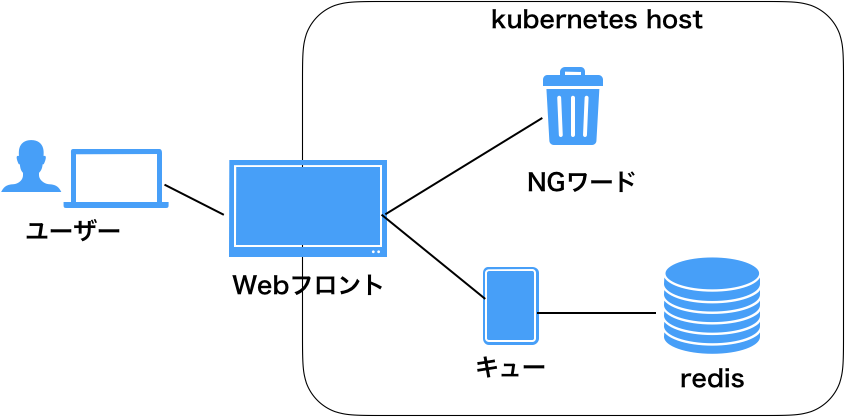
\includegraphics[width=10cm]{Web3tiers.png}

本システムにおける脆弱性は、以下の点があげられる。

\begin{itemize}
\item Webフロントからトークン取得し、k8sホストへの攻撃
\item Webフロントからシークレット取得し、他Podへの攻撃
\end{itemize}

対処方法としては、アプリケーションの設計とk8sホストの対策に分けられる。\\

アプリケーションの設計では、RBACをもとにユーザーへの権限付与を正確におこない、
一般ユーザーがWebフロントからトークンやシークレットなどの秘匿すべき情報を取得されないようにする。\\

k8sのホストでは、侵入を防ぐ対策と侵入されたときの被害の拡散を防ぐ方法がある。
侵入を防ぐ方法は、Seccomp,AppArmor,SELinuxの有効化や不要なプロセスの停止など一般的なセキュリティ強化策をとる。\\

また、被害の拡大防止には、以下が考えられる。

\begin{itemize}
\item 一般ユーザーでのアプリケーションの起動
\item rootファイルの書き込み不可
\item kernalの分割
\end{itemize}

攻撃の監視は、Pod間の通信を監視することで攻撃を発見することができる。
本発表では、\href{https://istio.io/}{Istio}による監視をとりあげた。
Istioは、以下の4つの機能があるアプリケーションである。

\begin{itemize}
\item サービス間のプロキシ
\item 通信の暗号化
\item 証明書の自動更新
\item ポッドのポリシーの一元管理
\end{itemize}

この機能によりポッド間の通信の管理をおこない不正アクセスを未然に防ぐことができる。\\

k8sのセキュリティ担保は、基盤だけではなくアプリケーション開発者も設計に気をくばらねばならない。
また、コンテナ独特のカーネルの共有という設計で新なリスクが増えたが、正しく対策をおこなえば攻撃の対策をおこなえることができる。
安全に素早くサービス提供するため、開発・運用それぞれがコンテナのセキュリティリスクを正確に把握し対策を施して、k8s上にシステムを構築する必要がある。
